% This file was created with tikzplotlib v0.10.1.
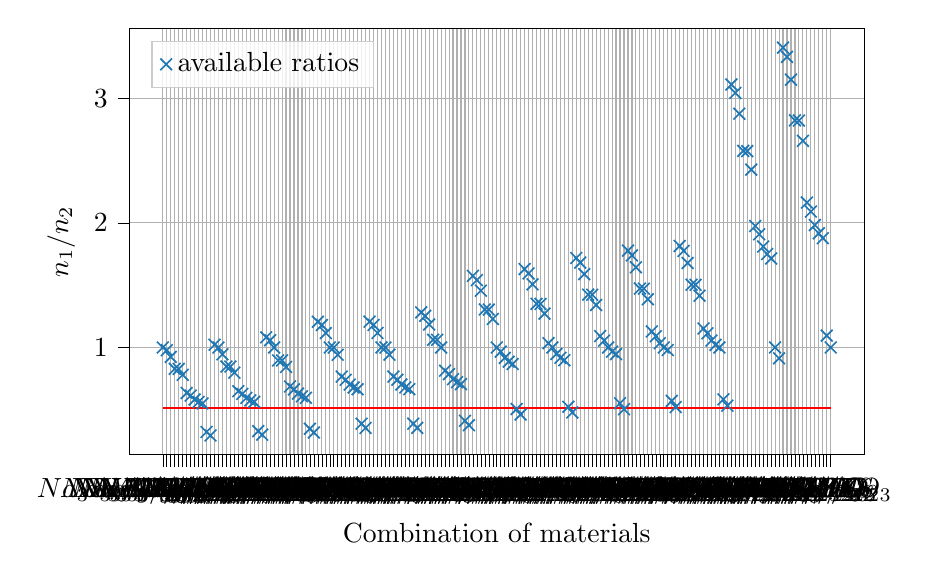
\begin{tikzpicture}

\definecolor{darkgray176}{RGB}{176,176,176}
\definecolor{lightgray204}{RGB}{204,204,204}
\definecolor{steelblue31119180}{RGB}{31,119,180}

\begin{axis}[
height=7cm,
legend cell align={left},
legend style={
  fill opacity=0.8,
  draw opacity=1,
  text opacity=1,
  at={(0.03,0.97)},
  anchor=north west,
  draw=lightgray204
},
tick align=outside,
tick pos=left,
width=0.9\textwidth,
x grid style={darkgray176},
xlabel={Combination of materials},
xmajorgrids,
xmin=-8.4, xmax=176.4,
xminorgrids,
xtick style={color=black},
xtick={0,1,2,3,4,5,6,7,8,9,10,11,12,13,14,15,16,17,18,19,20,21,22,23,24,25,26,27,28,29,30,31,32,33,34,35,36,37,38,39,40,41,42,43,44,45,46,47,48,49,50,51,52,53,54,55,56,57,58,59,60,61,62,63,64,65,66,67,68,69,70,71,72,73,74,75,76,77,78,79,80,81,82,83,84,85,86,87,88,89,90,91,92,93,94,95,96,97,98,99,100,101,102,103,104,105,106,107,108,109,110,111,112,113,114,115,116,117,118,119,120,121,122,123,124,125,126,127,128,129,130,131,132,133,134,135,136,137,138,139,140,141,142,143,144,145,146,147,148,149,150,151,152,153,154,155,156,157,158,159,160,161,162,163,164,165,166,167,168},
xtick={0,1,2,3,4,5,6,7,8,9,10,11,12,13,14,15,16,17,18,19,20,21,22,23,24,25,26,27,28,29,30,31,32,33,34,35,36,37,38,39,40,41,42,43,44,45,46,47,48,49,50,51,52,53,54,55,56,57,58,59,60,61,62,63,64,65,66,67,68,69,70,71,72,73,74,75,76,77,78,79,80,81,82,83,84,85,86,87,88,89,90,91,92,93,94,95,96,97,98,99,100,101,102,103,104,105,106,107,108,109,110,111,112,113,114,115,116,117,118,119,120,121,122,123,124,125,126,127,128,129,130,131,132,133,134,135,136,137,138,139,140,141,142,143,144,145,146,147,148,149,150,151,152,153,154,155,156,157,158,159,160,161,162,163,164,165,166,167,168},
xticklabels={
  \(\displaystyle Na_3AlF_6\)//\(\displaystyle Na_3AlF_6\),
  \(\displaystyle Na_3AlF_6\)//\(\displaystyle MgF_2\),
  \(\displaystyle Na_3AlF_6\)//\(\displaystyle SiO_2\),
  \(\displaystyle Na_3AlF_6\)//\(\displaystyle Al_2O_3\),
  \(\displaystyle Na_3AlF_6\)//\(\displaystyle CeF_3\),
  \(\displaystyle Na_3AlF_6\)//\(\displaystyle PbF_2\),
  \(\displaystyle Na_3AlF_6\)//\(\displaystyle Ta_2O_5\),
  \(\displaystyle Na_3AlF_6\)//\(\displaystyle ZrO_2\),
  \(\displaystyle Na_3AlF_6\)//\(\displaystyle ZnS\),
  \(\displaystyle Na_3AlF_6\)//\(\displaystyle TiO_2\),
  \(\displaystyle Na_3AlF_6\)//\(\displaystyle Bi_2O_3\),
  \(\displaystyle Na_3AlF_6\)//\(\displaystyle Ge\),
  \(\displaystyle Na_3AlF_6\)//\(\displaystyle Te\),
  \(\displaystyle MgF_2\)//\(\displaystyle Na_3AlF_6\),
  \(\displaystyle MgF_2\)//\(\displaystyle MgF_2\),
  \(\displaystyle MgF_2\)//\(\displaystyle SiO_2\),
  \(\displaystyle MgF_2\)//\(\displaystyle Al_2O_3\),
  \(\displaystyle MgF_2\)//\(\displaystyle CeF_3\),
  \(\displaystyle MgF_2\)//\(\displaystyle PbF_2\),
  \(\displaystyle MgF_2\)//\(\displaystyle Ta_2O_5\),
  \(\displaystyle MgF_2\)//\(\displaystyle ZrO_2\),
  \(\displaystyle MgF_2\)//\(\displaystyle ZnS\),
  \(\displaystyle MgF_2\)//\(\displaystyle TiO_2\),
  \(\displaystyle MgF_2\)//\(\displaystyle Bi_2O_3\),
  \(\displaystyle MgF_2\)//\(\displaystyle Ge\),
  \(\displaystyle MgF_2\)//\(\displaystyle Te\),
  \(\displaystyle SiO_2\)//\(\displaystyle Na_3AlF_6\),
  \(\displaystyle SiO_2\)//\(\displaystyle MgF_2\),
  \(\displaystyle SiO_2\)//\(\displaystyle SiO_2\),
  \(\displaystyle SiO_2\)//\(\displaystyle Al_2O_3\),
  \(\displaystyle SiO_2\)//\(\displaystyle CeF_3\),
  \(\displaystyle SiO_2\)//\(\displaystyle PbF_2\),
  \(\displaystyle SiO_2\)//\(\displaystyle Ta_2O_5\),
  \(\displaystyle SiO_2\)//\(\displaystyle ZrO_2\),
  \(\displaystyle SiO_2\)//\(\displaystyle ZnS\),
  \(\displaystyle SiO_2\)//\(\displaystyle TiO_2\),
  \(\displaystyle SiO_2\)//\(\displaystyle Bi_2O_3\),
  \(\displaystyle SiO_2\)//\(\displaystyle Ge\),
  \(\displaystyle SiO_2\)//\(\displaystyle Te\),
  \(\displaystyle Al_2O_3\)//\(\displaystyle Na_3AlF_6\),
  \(\displaystyle Al_2O_3\)//\(\displaystyle MgF_2\),
  \(\displaystyle Al_2O_3\)//\(\displaystyle SiO_2\),
  \(\displaystyle Al_2O_3\)//\(\displaystyle Al_2O_3\),
  \(\displaystyle Al_2O_3\)//\(\displaystyle CeF_3\),
  \(\displaystyle Al_2O_3\)//\(\displaystyle PbF_2\),
  \(\displaystyle Al_2O_3\)//\(\displaystyle Ta_2O_5\),
  \(\displaystyle Al_2O_3\)//\(\displaystyle ZrO_2\),
  \(\displaystyle Al_2O_3\)//\(\displaystyle ZnS\),
  \(\displaystyle Al_2O_3\)//\(\displaystyle TiO_2\),
  \(\displaystyle Al_2O_3\)//\(\displaystyle Bi_2O_3\),
  \(\displaystyle Al_2O_3\)//\(\displaystyle Ge\),
  \(\displaystyle Al_2O_3\)//\(\displaystyle Te\),
  \(\displaystyle CeF_3\)//\(\displaystyle Na_3AlF_6\),
  \(\displaystyle CeF_3\)//\(\displaystyle MgF_2\),
  \(\displaystyle CeF_3\)//\(\displaystyle SiO_2\),
  \(\displaystyle CeF_3\)//\(\displaystyle Al_2O_3\),
  \(\displaystyle CeF_3\)//\(\displaystyle CeF_3\),
  \(\displaystyle CeF_3\)//\(\displaystyle PbF_2\),
  \(\displaystyle CeF_3\)//\(\displaystyle Ta_2O_5\),
  \(\displaystyle CeF_3\)//\(\displaystyle ZrO_2\),
  \(\displaystyle CeF_3\)//\(\displaystyle ZnS\),
  \(\displaystyle CeF_3\)//\(\displaystyle TiO_2\),
  \(\displaystyle CeF_3\)//\(\displaystyle Bi_2O_3\),
  \(\displaystyle CeF_3\)//\(\displaystyle Ge\),
  \(\displaystyle CeF_3\)//\(\displaystyle Te\),
  \(\displaystyle PbF_2\)//\(\displaystyle Na_3AlF_6\),
  \(\displaystyle PbF_2\)//\(\displaystyle MgF_2\),
  \(\displaystyle PbF_2\)//\(\displaystyle SiO_2\),
  \(\displaystyle PbF_2\)//\(\displaystyle Al_2O_3\),
  \(\displaystyle PbF_2\)//\(\displaystyle CeF_3\),
  \(\displaystyle PbF_2\)//\(\displaystyle PbF_2\),
  \(\displaystyle PbF_2\)//\(\displaystyle Ta_2O_5\),
  \(\displaystyle PbF_2\)//\(\displaystyle ZrO_2\),
  \(\displaystyle PbF_2\)//\(\displaystyle ZnS\),
  \(\displaystyle PbF_2\)//\(\displaystyle TiO_2\),
  \(\displaystyle PbF_2\)//\(\displaystyle Bi_2O_3\),
  \(\displaystyle PbF_2\)//\(\displaystyle Ge\),
  \(\displaystyle PbF_2\)//\(\displaystyle Te\),
  \(\displaystyle Ta_2O_5\)//\(\displaystyle Na_3AlF_6\),
  \(\displaystyle Ta_2O_5\)//\(\displaystyle MgF_2\),
  \(\displaystyle Ta_2O_5\)//\(\displaystyle SiO_2\),
  \(\displaystyle Ta_2O_5\)//\(\displaystyle Al_2O_3\),
  \(\displaystyle Ta_2O_5\)//\(\displaystyle CeF_3\),
  \(\displaystyle Ta_2O_5\)//\(\displaystyle PbF_2\),
  \(\displaystyle Ta_2O_5\)//\(\displaystyle Ta_2O_5\),
  \(\displaystyle Ta_2O_5\)//\(\displaystyle ZrO_2\),
  \(\displaystyle Ta_2O_5\)//\(\displaystyle ZnS\),
  \(\displaystyle Ta_2O_5\)//\(\displaystyle TiO_2\),
  \(\displaystyle Ta_2O_5\)//\(\displaystyle Bi_2O_3\),
  \(\displaystyle Ta_2O_5\)//\(\displaystyle Ge\),
  \(\displaystyle Ta_2O_5\)//\(\displaystyle Te\),
  \(\displaystyle ZrO_2\)//\(\displaystyle Na_3AlF_6\),
  \(\displaystyle ZrO_2\)//\(\displaystyle MgF_2\),
  \(\displaystyle ZrO_2\)//\(\displaystyle SiO_2\),
  \(\displaystyle ZrO_2\)//\(\displaystyle Al_2O_3\),
  \(\displaystyle ZrO_2\)//\(\displaystyle CeF_3\),
  \(\displaystyle ZrO_2\)//\(\displaystyle PbF_2\),
  \(\displaystyle ZrO_2\)//\(\displaystyle Ta_2O_5\),
  \(\displaystyle ZrO_2\)//\(\displaystyle ZrO_2\),
  \(\displaystyle ZrO_2\)//\(\displaystyle ZnS\),
  \(\displaystyle ZrO_2\)//\(\displaystyle TiO_2\),
  \(\displaystyle ZrO_2\)//\(\displaystyle Bi_2O_3\),
  \(\displaystyle ZrO_2\)//\(\displaystyle Ge\),
  \(\displaystyle ZrO_2\)//\(\displaystyle Te\),
  \(\displaystyle ZnS\)//\(\displaystyle Na_3AlF_6\),
  \(\displaystyle ZnS\)//\(\displaystyle MgF_2\),
  \(\displaystyle ZnS\)//\(\displaystyle SiO_2\),
  \(\displaystyle ZnS\)//\(\displaystyle Al_2O_3\),
  \(\displaystyle ZnS\)//\(\displaystyle CeF_3\),
  \(\displaystyle ZnS\)//\(\displaystyle PbF_2\),
  \(\displaystyle ZnS\)//\(\displaystyle Ta_2O_5\),
  \(\displaystyle ZnS\)//\(\displaystyle ZrO_2\),
  \(\displaystyle ZnS\)//\(\displaystyle ZnS\),
  \(\displaystyle ZnS\)//\(\displaystyle TiO_2\),
  \(\displaystyle ZnS\)//\(\displaystyle Bi_2O_3\),
  \(\displaystyle ZnS\)//\(\displaystyle Ge\),
  \(\displaystyle ZnS\)//\(\displaystyle Te\),
  \(\displaystyle TiO_2\)//\(\displaystyle Na_3AlF_6\),
  \(\displaystyle TiO_2\)//\(\displaystyle MgF_2\),
  \(\displaystyle TiO_2\)//\(\displaystyle SiO_2\),
  \(\displaystyle TiO_2\)//\(\displaystyle Al_2O_3\),
  \(\displaystyle TiO_2\)//\(\displaystyle CeF_3\),
  \(\displaystyle TiO_2\)//\(\displaystyle PbF_2\),
  \(\displaystyle TiO_2\)//\(\displaystyle Ta_2O_5\),
  \(\displaystyle TiO_2\)//\(\displaystyle ZrO_2\),
  \(\displaystyle TiO_2\)//\(\displaystyle ZnS\),
  \(\displaystyle TiO_2\)//\(\displaystyle TiO_2\),
  \(\displaystyle TiO_2\)//\(\displaystyle Bi_2O_3\),
  \(\displaystyle TiO_2\)//\(\displaystyle Ge\),
  \(\displaystyle TiO_2\)//\(\displaystyle Te\),
  \(\displaystyle Bi_2O_3\)//\(\displaystyle Na_3AlF_6\),
  \(\displaystyle Bi_2O_3\)//\(\displaystyle MgF_2\),
  \(\displaystyle Bi_2O_3\)//\(\displaystyle SiO_2\),
  \(\displaystyle Bi_2O_3\)//\(\displaystyle Al_2O_3\),
  \(\displaystyle Bi_2O_3\)//\(\displaystyle CeF_3\),
  \(\displaystyle Bi_2O_3\)//\(\displaystyle PbF_2\),
  \(\displaystyle Bi_2O_3\)//\(\displaystyle Ta_2O_5\),
  \(\displaystyle Bi_2O_3\)//\(\displaystyle ZrO_2\),
  \(\displaystyle Bi_2O_3\)//\(\displaystyle ZnS\),
  \(\displaystyle Bi_2O_3\)//\(\displaystyle TiO_2\),
  \(\displaystyle Bi_2O_3\)//\(\displaystyle Bi_2O_3\),
  \(\displaystyle Bi_2O_3\)//\(\displaystyle Ge\),
  \(\displaystyle Bi_2O_3\)//\(\displaystyle Te\),
  \(\displaystyle Ge\)//\(\displaystyle Na_3AlF_6\),
  \(\displaystyle Ge\)//\(\displaystyle MgF_2\),
  \(\displaystyle Ge\)//\(\displaystyle SiO_2\),
  \(\displaystyle Ge\)//\(\displaystyle Al_2O_3\),
  \(\displaystyle Ge\)//\(\displaystyle CeF_3\),
  \(\displaystyle Ge\)//\(\displaystyle PbF_2\),
  \(\displaystyle Ge\)//\(\displaystyle Ta_2O_5\),
  \(\displaystyle Ge\)//\(\displaystyle ZrO_2\),
  \(\displaystyle Ge\)//\(\displaystyle ZnS\),
  \(\displaystyle Ge\)//\(\displaystyle TiO_2\),
  \(\displaystyle Ge\)//\(\displaystyle Bi_2O_3\),
  \(\displaystyle Ge\)//\(\displaystyle Ge\),
  \(\displaystyle Ge\)//\(\displaystyle Te\),
  \(\displaystyle Te\)//\(\displaystyle Na_3AlF_6\),
  \(\displaystyle Te\)//\(\displaystyle MgF_2\),
  \(\displaystyle Te\)//\(\displaystyle SiO_2\),
  \(\displaystyle Te\)//\(\displaystyle Al_2O_3\),
  \(\displaystyle Te\)//\(\displaystyle CeF_3\),
  \(\displaystyle Te\)//\(\displaystyle PbF_2\),
  \(\displaystyle Te\)//\(\displaystyle Ta_2O_5\),
  \(\displaystyle Te\)//\(\displaystyle ZrO_2\),
  \(\displaystyle Te\)//\(\displaystyle ZnS\),
  \(\displaystyle Te\)//\(\displaystyle TiO_2\),
  \(\displaystyle Te\)//\(\displaystyle Bi_2O_3\),
  \(\displaystyle Te\)//\(\displaystyle Ge\),
  \(\displaystyle Te\)//\(\displaystyle Te\)
},
xticklabels={$Na_3AlF_6$//$Na_3AlF_6$,$Na_3AlF_6$//$MgF_2$,$Na_3AlF_6$//$SiO_2$,$Na_3AlF_6$//$Al_2O_3$,$Na_3AlF_6$//$CeF_3$,$Na_3AlF_6$//$PbF_2$,$Na_3AlF_6$//$Ta_2O_5$,$Na_3AlF_6$//$ZrO_2$,$Na_3AlF_6$//$ZnS$,$Na_3AlF_6$//$TiO_2$,$Na_3AlF_6$//$Bi_2O_3$,$Na_3AlF_6$//$Ge$,$Na_3AlF_6$//$Te$,$MgF_2$//$Na_3AlF_6$,$MgF_2$//$MgF_2$,$MgF_2$//$SiO_2$,$MgF_2$//$Al_2O_3$,$MgF_2$//$CeF_3$,$MgF_2$//$PbF_2$,$MgF_2$//$Ta_2O_5$,$MgF_2$//$ZrO_2$,$MgF_2$//$ZnS$,$MgF_2$//$TiO_2$,$MgF_2$//$Bi_2O_3$,$MgF_2$//$Ge$,$MgF_2$//$Te$,$SiO_2$//$Na_3AlF_6$,$SiO_2$//$MgF_2$,$SiO_2$//$SiO_2$,$SiO_2$//$Al_2O_3$,$SiO_2$//$CeF_3$,$SiO_2$//$PbF_2$,$SiO_2$//$Ta_2O_5$,$SiO_2$//$ZrO_2$,$SiO_2$//$ZnS$,$SiO_2$//$TiO_2$,$SiO_2$//$Bi_2O_3$,$SiO_2$//$Ge$,$SiO_2$//$Te$,$Al_2O_3$//$Na_3AlF_6$,$Al_2O_3$//$MgF_2$,$Al_2O_3$//$SiO_2$,$Al_2O_3$//$Al_2O_3$,$Al_2O_3$//$CeF_3$,$Al_2O_3$//$PbF_2$,$Al_2O_3$//$Ta_2O_5$,$Al_2O_3$//$ZrO_2$,$Al_2O_3$//$ZnS$,$Al_2O_3$//$TiO_2$,$Al_2O_3$//$Bi_2O_3$,$Al_2O_3$//$Ge$,$Al_2O_3$//$Te$,$CeF_3$//$Na_3AlF_6$,$CeF_3$//$MgF_2$,$CeF_3$//$SiO_2$,$CeF_3$//$Al_2O_3$,$CeF_3$//$CeF_3$,$CeF_3$//$PbF_2$,$CeF_3$//$Ta_2O_5$,$CeF_3$//$ZrO_2$,$CeF_3$//$ZnS$,$CeF_3$//$TiO_2$,$CeF_3$//$Bi_2O_3$,$CeF_3$//$Ge$,$CeF_3$//$Te$,$PbF_2$//$Na_3AlF_6$,$PbF_2$//$MgF_2$,$PbF_2$//$SiO_2$,$PbF_2$//$Al_2O_3$,$PbF_2$//$CeF_3$,$PbF_2$//$PbF_2$,$PbF_2$//$Ta_2O_5$,$PbF_2$//$ZrO_2$,$PbF_2$//$ZnS$,$PbF_2$//$TiO_2$,$PbF_2$//$Bi_2O_3$,$PbF_2$//$Ge$,$PbF_2$//$Te$,$Ta_2O_5$//$Na_3AlF_6$,$Ta_2O_5$//$MgF_2$,$Ta_2O_5$//$SiO_2$,$Ta_2O_5$//$Al_2O_3$,$Ta_2O_5$//$CeF_3$,$Ta_2O_5$//$PbF_2$,$Ta_2O_5$//$Ta_2O_5$,$Ta_2O_5$//$ZrO_2$,$Ta_2O_5$//$ZnS$,$Ta_2O_5$//$TiO_2$,$Ta_2O_5$//$Bi_2O_3$,$Ta_2O_5$//$Ge$,$Ta_2O_5$//$Te$,$ZrO_2$//$Na_3AlF_6$,$ZrO_2$//$MgF_2$,$ZrO_2$//$SiO_2$,$ZrO_2$//$Al_2O_3$,$ZrO_2$//$CeF_3$,$ZrO_2$//$PbF_2$,$ZrO_2$//$Ta_2O_5$,$ZrO_2$//$ZrO_2$,$ZrO_2$//$ZnS$,$ZrO_2$//$TiO_2$,$ZrO_2$//$Bi_2O_3$,$ZrO_2$//$Ge$,$ZrO_2$//$Te$,$ZnS$//$Na_3AlF_6$,$ZnS$//$MgF_2$,$ZnS$//$SiO_2$,$ZnS$//$Al_2O_3$,$ZnS$//$CeF_3$,$ZnS$//$PbF_2$,$ZnS$//$Ta_2O_5$,$ZnS$//$ZrO_2$,$ZnS$//$ZnS$,$ZnS$//$TiO_2$,$ZnS$//$Bi_2O_3$,$ZnS$//$Ge$,$ZnS$//$Te$,$TiO_2$//$Na_3AlF_6$,$TiO_2$//$MgF_2$,$TiO_2$//$SiO_2$,$TiO_2$//$Al_2O_3$,$TiO_2$//$CeF_3$,$TiO_2$//$PbF_2$,$TiO_2$//$Ta_2O_5$,$TiO_2$//$ZrO_2$,$TiO_2$//$ZnS$,$TiO_2$//$TiO_2$,$TiO_2$//$Bi_2O_3$,$TiO_2$//$Ge$,$TiO_2$//$Te$,$Bi_2O_3$//$Na_3AlF_6$,$Bi_2O_3$//$MgF_2$,$Bi_2O_3$//$SiO_2$,$Bi_2O_3$//$Al_2O_3$,$Bi_2O_3$//$CeF_3$,$Bi_2O_3$//$PbF_2$,$Bi_2O_3$//$Ta_2O_5$,$Bi_2O_3$//$ZrO_2$,$Bi_2O_3$//$ZnS$,$Bi_2O_3$//$TiO_2$,$Bi_2O_3$//$Bi_2O_3$,$Bi_2O_3$//$Ge$,$Bi_2O_3$//$Te$,$Ge$//$Na_3AlF_6$,$Ge$//$MgF_2$,$Ge$//$SiO_2$,$Ge$//$Al_2O_3$,$Ge$//$CeF_3$,$Ge$//$PbF_2$,$Ge$//$Ta_2O_5$,$Ge$//$ZrO_2$,$Ge$//$ZnS$,$Ge$//$TiO_2$,$Ge$//$Bi_2O_3$,$Ge$//$Ge$,$Ge$//$Te$,$Te$//$Na_3AlF_6$,$Te$//$MgF_2$,$Te$//$SiO_2$,$Te$//$Al_2O_3$,$Te$//$CeF_3$,$Te$//$PbF_2$,$Te$//$Ta_2O_5$,$Te$//$ZrO_2$,$Te$//$ZnS$,$Te$//$TiO_2$,$Te$//$Bi_2O_3$,$Te$//$Ge$,$Te$//$Te$},
y grid style={darkgray176},
ylabel={\(\displaystyle n_1/n_2\)},
ymajorgrids,
ymin=0.137781803542673, ymax=3.5631038647343,
yminorgrids,
ytick style={color=black}
]
\addplot [semithick, steelblue31119180, mark=x, mark size=3, mark options={solid}, only marks]
table {%
0 1
1 0.978260869565218
2 0.924657534246575
3 0.828729281767956
4 0.828220858895706
5 0.780346820809249
6 0.634995296331138
7 0.613636363636364
8 0.581896551724138
9 0.5625
10 0.551020408163265
11 0.321428571428571
12 0.293478260869565
13 1.02222222222222
14 1
15 0.945205479452055
16 0.847145488029466
17 0.846625766871166
18 0.797687861271676
19 0.649106302916275
20 0.627272727272727
21 0.594827586206897
22 0.575
23 0.563265306122449
24 0.328571428571429
25 0.3
26 1.08148148148148
27 1.05797101449275
28 1
29 0.896255371393493
30 0.895705521472393
31 0.84393063583815
32 0.686735653809972
33 0.663636363636364
34 0.629310344827586
35 0.608333333333333
36 0.595918367346939
37 0.347619047619048
38 0.317391304347826
39 1.20666666666667
40 1.1804347826087
41 1.11575342465753
42 1
43 0.999386503067485
44 0.941618497109827
45 0.766227657572907
46 0.740454545454545
47 0.702155172413793
48 0.67875
49 0.664897959183673
50 0.387857142857143
51 0.354130434782609
52 1.20740740740741
53 1.18115942028985
54 1.11643835616438
55 1.00061387354205
56 1
57 0.942196531791907
58 0.766698024459078
59 0.740909090909091
60 0.702586206896552
61 0.679166666666667
62 0.665306122448979
63 0.388095238095238
64 0.354347826086957
65 1.28148148148148
66 1.2536231884058
67 1.18493150684932
68 1.06200122774708
69 1.06134969325153
70 1
71 0.813734713076199
72 0.786363636363636
73 0.745689655172414
74 0.720833333333333
75 0.706122448979592
76 0.411904761904762
77 0.376086956521739
78 1.57481481481481
79 1.54057971014493
80 1.45616438356164
81 1.30509515039902
82 1.30429447852761
83 1.22890173410405
84 1
85 0.966363636363636
86 0.916379310344828
87 0.885833333333333
88 0.867755102040816
89 0.506190476190476
90 0.462173913043478
91 1.62962962962963
92 1.59420289855072
93 1.50684931506849
94 1.35052179251074
95 1.34969325153374
96 1.27167630057803
97 1.03480714957667
98 1
99 0.948275862068966
100 0.916666666666667
101 0.897959183673469
102 0.523809523809524
103 0.478260869565217
104 1.71851851851852
105 1.68115942028985
106 1.58904109589041
107 1.42418661755678
108 1.42331288343558
109 1.34104046242775
110 1.09125117591722
111 1.05454545454545
112 1
113 0.966666666666667
114 0.946938775510204
115 0.552380952380952
116 0.504347826086956
117 1.77777777777778
118 1.73913043478261
119 1.64383561643836
120 1.47329650092081
121 1.47239263803681
122 1.38728323699422
123 1.12888052681091
124 1.09090909090909
125 1.03448275862069
126 1
127 0.979591836734694
128 0.571428571428571
129 0.521739130434783
130 1.81481481481481
131 1.77536231884058
132 1.67808219178082
133 1.50399017802333
134 1.50306748466258
135 1.41618497109827
136 1.15239887111947
137 1.11363636363636
138 1.05603448275862
139 1.02083333333333
140 1
141 0.583333333333333
142 0.532608695652174
143 3.11111111111111
144 3.04347826086957
145 2.87671232876712
146 2.57826887661142
147 2.57668711656442
148 2.42774566473988
149 1.9755409219191
150 1.90909090909091
151 1.81034482758621
152 1.75
153 1.71428571428571
154 1
155 0.91304347826087
156 3.40740740740741
157 3.33333333333333
158 3.15068493150685
159 2.82381829343155
160 2.82208588957055
161 2.65895953757225
162 2.16368767638758
163 2.09090909090909
164 1.98275862068966
165 1.91666666666667
166 1.87755102040816
167 1.0952380952381
168 1
};
\addlegendentry{available ratios}
\path [draw=red, semithick]
(axis cs:0,0.512989176042577)
--(axis cs:168,0.512989176042577);

\end{axis}

\end{tikzpicture}
